The main topic of this thesis is Partially Observable Markov Decision Processes (POMDPs).
The practical use of this model has been criticized in Introduction, 
however it sums up accurately the principal features of a robotic system.
Next, Possibility Theory is presented
in order to introduce Qualitative Possibilistic Markov Decision Processes ($\pi$-MDPs)
and Partially Observable ones ($\pi$-POMDPs) which are the starting point
of this work.

\subsection{Partially Observable Markov Decision Process} \label{section_POMDP}

\begin{figure}[!t]
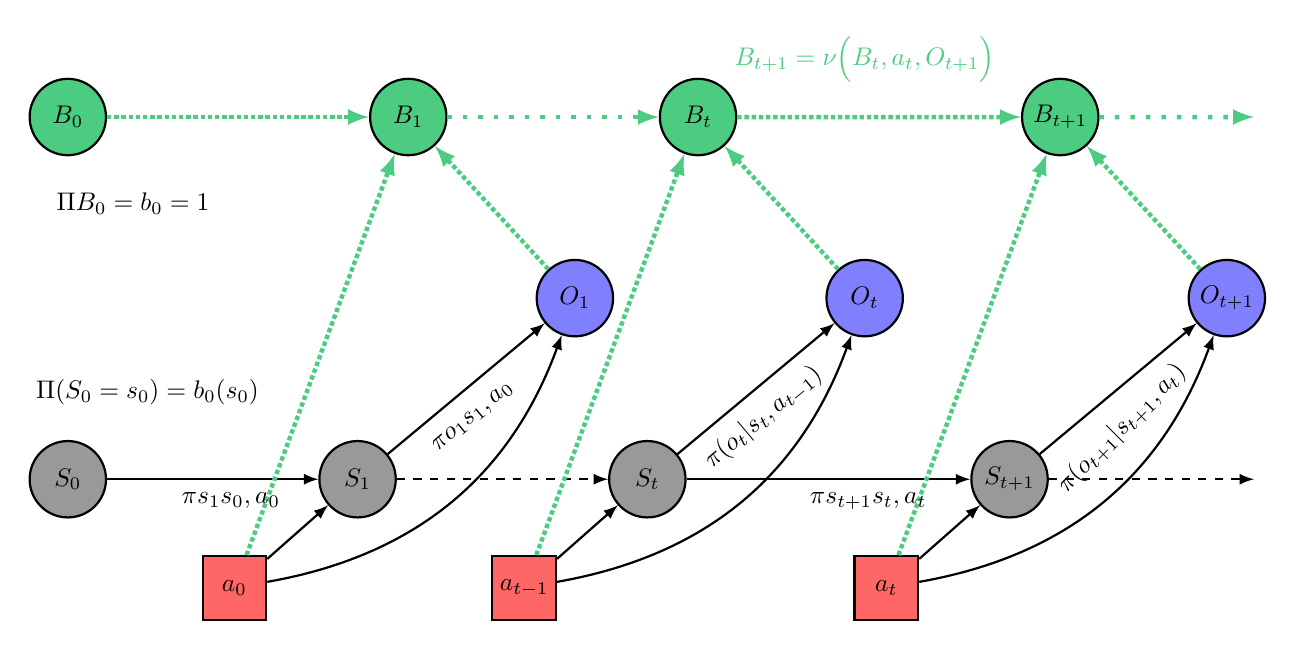
\begin{tikzpicture}[transform shape,scale=0.92]
%% vertex shape and color
\tikzstyle{vertex}=[circle,fill=black!40,minimum size=30pt,inner sep=0pt,draw=black,thick]
\tikzstyle{avertex}=[rectangle,fill=red!60,minimum size=25pt,inner sep=0pt,draw=black,thick]
\tikzstyle{rvertex}=[fill=yellow!60,decision=3,inner sep=-1pt,minimum size=35pt,draw=black,thick]
\definecolor{darkgreen}{rgb}{0.3,0.8,0.5}
\tikzstyle{bvertex}=[circle,fill=darkgreen,minimum size=30pt,inner sep=0pt,draw=black,thick]
\tikzstyle{overtex}=[circle,fill=blue!50,minimum size=30pt,inner sep=0pt,draw=black,thick]

%% nodes
% states
\foreach \name/\x in {S_0/0,S_1/4,S_t/8, S_{t+1}/13}
\node[vertex] (G-\name) at (\x,0) {$\name$};
\node (G-end) at (16.5,0) {};
% actions
\foreach \name/\x in {a_0/0,a_{t-1}/4,a_t/9}
\node[avertex] (G-\name) at (\x+2.3,-1.5) {$\name$};
% observations
\foreach \name/\x in {O_1/4,O_t/8,O_{t+1}/13}
\node[overtex] (G-\name) at (\x+3,2.5) {$\name$};
% beliefs
\foreach \name/\x in {B_0/0,B_1/4.7,B_t/8.7,B_{t+1}/13.7}
\node[bvertex] (G-\name) at (\x,5) {$\name$};
\node (G-B-end) at (16.5,5) {};

%% arrows
% states
\foreach \from/\to in {S_0/S_1,S_t/S_{t+1}}
\draw[->,>=latex,thick] (G-\from) -- (G-\to);
\foreach \from/\to in {S_1/S_t,S_{t+1}/end}
\draw[->,>=latex,dashed,thick] (G-\from) -- (G-\to);
% actions
\foreach \from/\to in {a_0/S_1,a_{t-1}/S_t,a_t/S_{t+1}}
\draw[->,>=latex,thick] (G-\from) -- (G-\to);
\foreach \from/\to in {a_0/O_1,a_{t-1}/O_t,a_t/O_{t+1}}
\draw[->,>=latex,thick] (G-\from) to[bend right]  (G-\to);
% rewards
% observations
\foreach \from/\to in {S_1/O_1,S_t/O_t,S_{t+1}/O_{t+1}}
\draw[->,>=latex,thick] (G-\from) -- (G-\to);
% beliefs
\foreach \from/\to in {B_0/B_1,B_t/B_{t+1}}
\draw[->,>=latex,color=darkgreen,ultra thick,densely dotted] (G-\from) -- (G-\to);
\foreach \from/\to in {B_1/B_t,B_{t+1}/B-end}
\draw[->,>=latex,color=darkgreen,ultra thick,loosely dotted] (G-\from) to (G-\to);
\foreach \from/\to in {O_1/B_1,O_t/B_t,O_{t+1}/B_{t+1}}
\draw[->,>=latex,color=darkgreen,ultra thick,densely dotted] (G-\from) to (G-\to);

\foreach \from/\to in {a_0/B_1,a_{t-1}/B_t,a_t/B_{t+1}}
\draw[->,>=latex,color=darkgreen,ultra thick,densely dotted] (G-\from) to (G-\to);

%%%%%%%%%%%%%%%%%%%%%%%%%%%%%%%%%%%%%%%%%%%%%%%%%%%%%%%%%%%%%%%%%%%%%%%%
% probabilities
% state transition
\node (proba1) at (2.25,-0.3) {$\pi \paren{ s_{1} \sachant s_{0}, a_0}$};
\node (probat) at (11.05,-0.3) {$\pi \paren{ s_{t+1} \sachant s_t, a_t}$};
% observations
\node (probo1) at (5.6,0.85) [rotate=40] {$\pi \paren{o_1 \sachant s_1,a_0}$};
\node (probot) at (9.6,0.85) [rotate=40] {$\pi ( o_t \vert s_t,a_{t-1} )$};
\node (probotp1) at (14.55,0.7) [rotate=45] {$\pi ( o_{t+1} \vert s_{t+1},a_{t})$};
% bel
\node (pbb) at (11,5.8) [color=darkgreen] {$B_{t+1} = \nu\Big(B_{t},a_t,O_{t+1}\Big)$};
\node (pbb) at (0.9,3.8)  {$\Pi \paren{B_0 = b_0} = 1$};% \mathds{1}_{ \set{ b = b_0}}(b)$};
\node (pbb) at (1.1,1.2) {$\Pi(S_0 = s_0) = b_0(s_0)$};
\end{tikzpicture}

\caption[Influence Diagram of a POMDP and its belief updating process]{
Influence Diagram of a POMDP and its belief updating process:
black circles represent successive system states $S_t$,
blue ones represent successive observations $O_t$,
red squares are selected actions $a_t$,
and yellow diamonds are the associated rewards.
Green circles at the top of the figure are the successive belief states 
$B_t$ constituting the belief updating process,
computed using the update $B_{t+1} = u(B_t,a_t,O_{t+1})$.
Just like the wavy lines leading to rewards, 
the green dotted lines represent a deterministic influence.
The Bayesian Network resulting from removing belief states and rewards, 
asserts that $\forall t \geqslant 1$, $S_{t+1} \perp\!\!\!\perp \set{ S_{0},S_1, O_1, \ldots, S_{t-1}, O_{t-1} } \vert \set{S_t,A_t}$,
where $A_t$ represents the action at time step $t$ seen as a random variable.
As well, $\forall t \geqslant 1$, $O_{t}$ is independent from all other variables 
conditional on $\set{S_t, A_t}$.}
\label{POMDP} 
\end{figure}

